\textbf{Постановка задачи}
В качестве выносимых на защиту положений диссертационной работы нами 
выдвигается модификация модели прогнозирования численности наркозависимых с
помощью нечеткой логики, а также приложение для проведения необходимых расчетов.
Приложение по своей структуре должно соответствовать стандартам, принятым в
МАСП <<Прогноз>>.

Программный компонент прогнозирования численности наркозависимых предназначен
для поддержки принятия управленческих решений Губернатором Санкт-Петербурга,
Правительством Санкт-Петербурга, Антинаркотической комиссией, руководителями
ИОГВ по определению приоритетных направлений реализации антирнаркотической
политики Санкт-Петербурга.

Программа должна обеспечивать:
\begin{itemize}
    \item Загрузку исходных данных в виде файлов формата CSV, XLSX, а также с
        помощью API ИС ИАО, ИС <<Антинар>>;
    \item Очистку и нормализацию данных;
    \item Настройку параметров моделирования;
    \item Произведение необходимых расчетов;
    \item Генерацию аналитических продуктов;
    \item Визуализацию аналитических продуктов в виде таблиц, графиков, базы
        нечетких правил.
\end{itemize}

\textbf{Фреймворк Shiny как инструмент для разработки веб-приложений в области
статистики.}
Shiny --- фреймворк для программирования интерактивных веб-приложений на языке 
статистического программирования R.

Приложения для Shiny состоят из двух компонент:
\begin{itemize}
    \item скрипт пользовательского интерфейса;
    \item скрипт серверной части.
\end{itemize}
Скрипт пользовательского интерфейса контролирует расположение элементов и
внешний вид приложения (рис. ~\ref{figure:layouts}). 

\begin{figure}[bhtp]
    \centering
    \includetextwidthgraphics{images/layouts.png}
    \caption{Варианты расположения элементов интерфейса в Shiny}		
    \label{figure:layouts}
\end{figure}
Серверный скрипт содержит инструкции, которые требуются компьютеру для построения 
приложения.

Важной особенностью фреймворка Shiny, обеспечивающим создание на его основе
интерактивных приложений, является применяемая в нём модель реактивного
программирования. В ней выделяется три типа объектов: \textbf{реактивные
    источники}, \textbf{реактивные проводники}, и \textbf{реактивные приемники}.
Простейшая реактивная программа включает в свою структуру один источник и один
приемник. В приложении на Shiny источником обычно является пользовательский ввод
через интерфейс браузера.  Источник сигнализирует дочерним узлам о необходимости
повторно исполнить код. Реактивным приемником обычно является нечто, выводящееся
в окно браузера, например график или таблица с числовыми значениями.  Реактивный
источник может быть подключен ко многим приемникам, и наоборот.  Приемнику могут
поступать запросы на исполнение, и он может отсылать запросы на исполнение
объектам родительского уровня. В качестве промежуточного реактивного компонента
между источником и приемником может выступать реактивный проводник. Проводник
может быть зависимым и иметь зависимых. Иначе говоря, он может быть как
родительским, так и дочерним узлом в графе реактивной структуры приложения.
Источники могут быть только родительскими, а приемники только дочерними узлами.
Типичным применением реактивного проводника является инкапусляция медленных или
вычислительноемких операций.

\textbf{Анализ логической структуры программы.}
С учетом выдвинутых требований к разработке программы и возможностей фреймворка
Shiny и библиотеки frbs, необходимо в первую очередь определиться с вариантами
использования программы с точки зрения конечного пользователя: аналитика либо
иного представителя ОГВ. Аналитик, прежде всего, должен определиться с
параметрами моделирования, в которые входят как исследуемые показатели
социально-экономического развития города, так и собственно параметры
математической модели (рис. ~\ref{figure:usecase1}). Но основной интерес для
аналитика представляют аналитические продукты, генерирумые моделью: прогнозные
значения, оценки ошибок прогнозирования, база нечетких продукционных правил,
которые отображаются в виде графиков и таблиц.
\begin{figure}[bhtp]
    \includetextwidthgraphics{images/usecase1.png}
    \caption{Диаграмма вариантов использования}		
    \label{figure:usecase1}
\end{figure}
Для реализации принципа кроссплатформенности и снижения нагрузки на аппаратное
обеспечение конечного пользователя целесообразно обратиться к архитектуре
<<клиент-сервер>>, тем самым предоставляя пользователю доступ лишь к <<тонкому
клиенту>>, а ресурсоемкие вычисления производить на сервере (рис.
~\ref{figure:sequence1}, ~\ref{figure:sequence2}). Моделирование предполагает
строгое соблюдение последовательности действий: сначала настройка параметров
модели, затем генерация результатов. Однако, с точки зрения юзабилити, имеет
смысл создать набор параметров по умолчанию для снижения порога вхождения для
нового пользователя. Другим полезным свойством должна быть возможность менять
параметры модели <<на лету>> для обечпечения итеративной настройки и
постепенного приближения пользователя к достижению целей моделирования.
\begin{figure}[bhtp]
    \includetextwidthgraphics{images/sequence1.png}
    \caption{Диаграмма последовательности №1}		
    \label{figure:sequence1}
\end{figure}

\begin{figure}[bhtp]
    \includetextwidthgraphics{images/sequence2.png}
    \caption{Диаграмма последовательности №2}		
    \label{figure:sequence2}
\end{figure}

\textbf{Описание функций  и интерфейса программы.}
Серверная часть приложения базируется на пакете frbs языка статистического
программирования R. Данный пакет предоставляет средства для построения
и использования систем на основе нечетких правил. В частности, это широкий
арсенал методов обучения модели: эвристические процедуры, нейро-нечеткие методы,
кластеризация, генетические алгоритмы и др. Данный пакет разработан учеными
Гранадского университета и ставит своей целью стать стандартным пакетом для
нечеткого моделирования в R.

Интерфейс приложения построен по схеме sidebarLayout+tabPanel. Общим для всех
вкладок является боковая секция, где предланается выбрать входные данные
(предикторы) и зависимую переменную (предиктанд). Также на ней устанавливается
горизонт прогнозирования и обучающий алгоритм. На первой вкладке
(рис.~\ref{figure:screenshot1}) показывается график с результатами
моделирования.  

\begin{figure}[bhtp]
    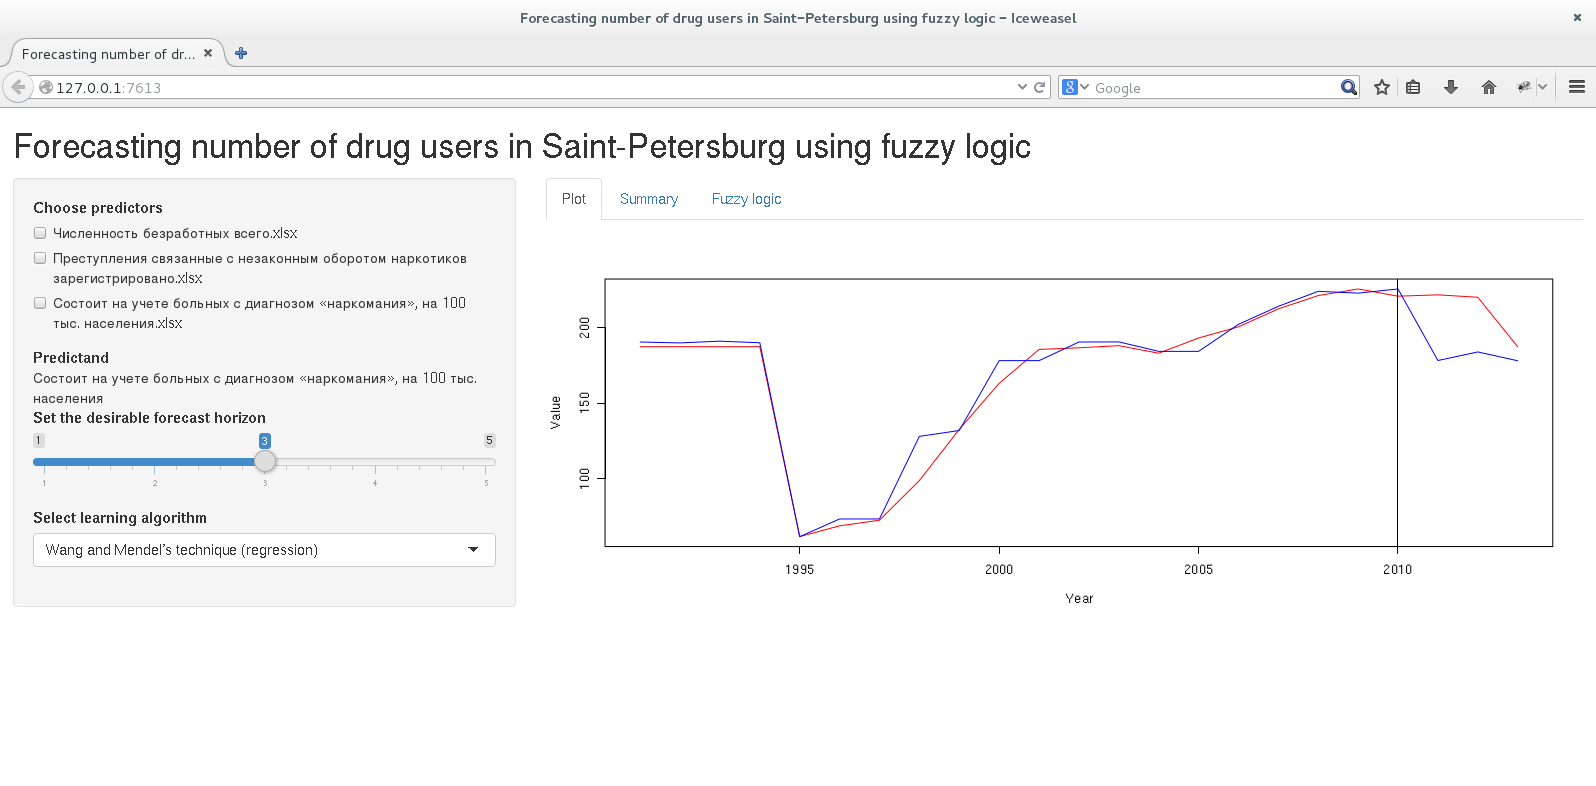
\includegraphics{images/screenshot1.png}
    \caption{Вкладка 1. График}		
    \label{figure:screenshot1}
\end{figure}

На второй вкладке (рис.~\ref{figure:screenshot2}) показаны таблицы для оценки
точности моделирования. Во-первых, это таблица, в которой приведены эмпирические
значения и значения модели для сравнения. Во-вторых, это таблица с оценками
точности прогнозирования по методам среднеквадратичного отклонения, корня из
среднеквадратичной ошибки, симметрическая средняя абсолютная ошибка в процентах.

\begin{figure}[bhtp]
    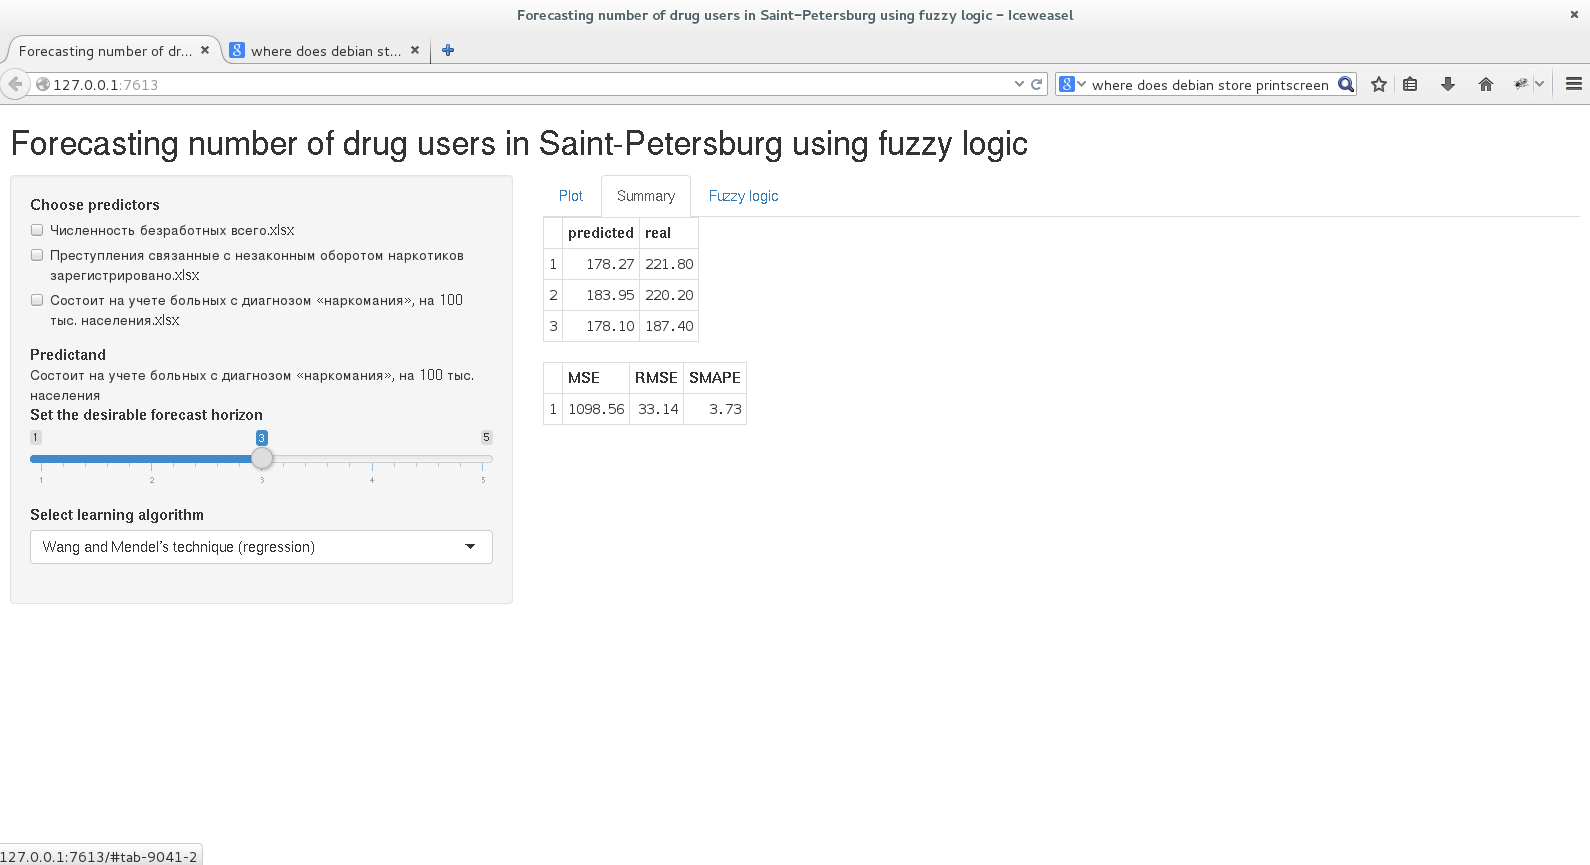
\includegraphics{images/screenshot2.png}
    \caption{Вкладка 2. Таблицы оценки точности}		
    \label{figure:screenshot2}
\end{figure}

На третьей вкладке (рис.~\ref{figure:screenshot3}) приведены сведения о нечеткой
модели. К ним относятся: название модели, наименование обучающего алгоритма,
названия используемых показателей, интервалы данных, тип нечеткой модели, тип
функции принадлежности, тип оператора конъюнкции, тип оператора дизъюнкции, тип
оператора дефаззификации, тип функции импликации, названия лингвистических
термов входных переменных, названия лингвистических термов выходной переменной,
нормализованные значения параметров функций принадлежности входных переменных,
нечеткие правила типа <<ЕСЛИ-ТО>>, специфические параметры: линейные уравнения,
веса правил, центры кластеров и др.

\begin{figure}[bhtp]
    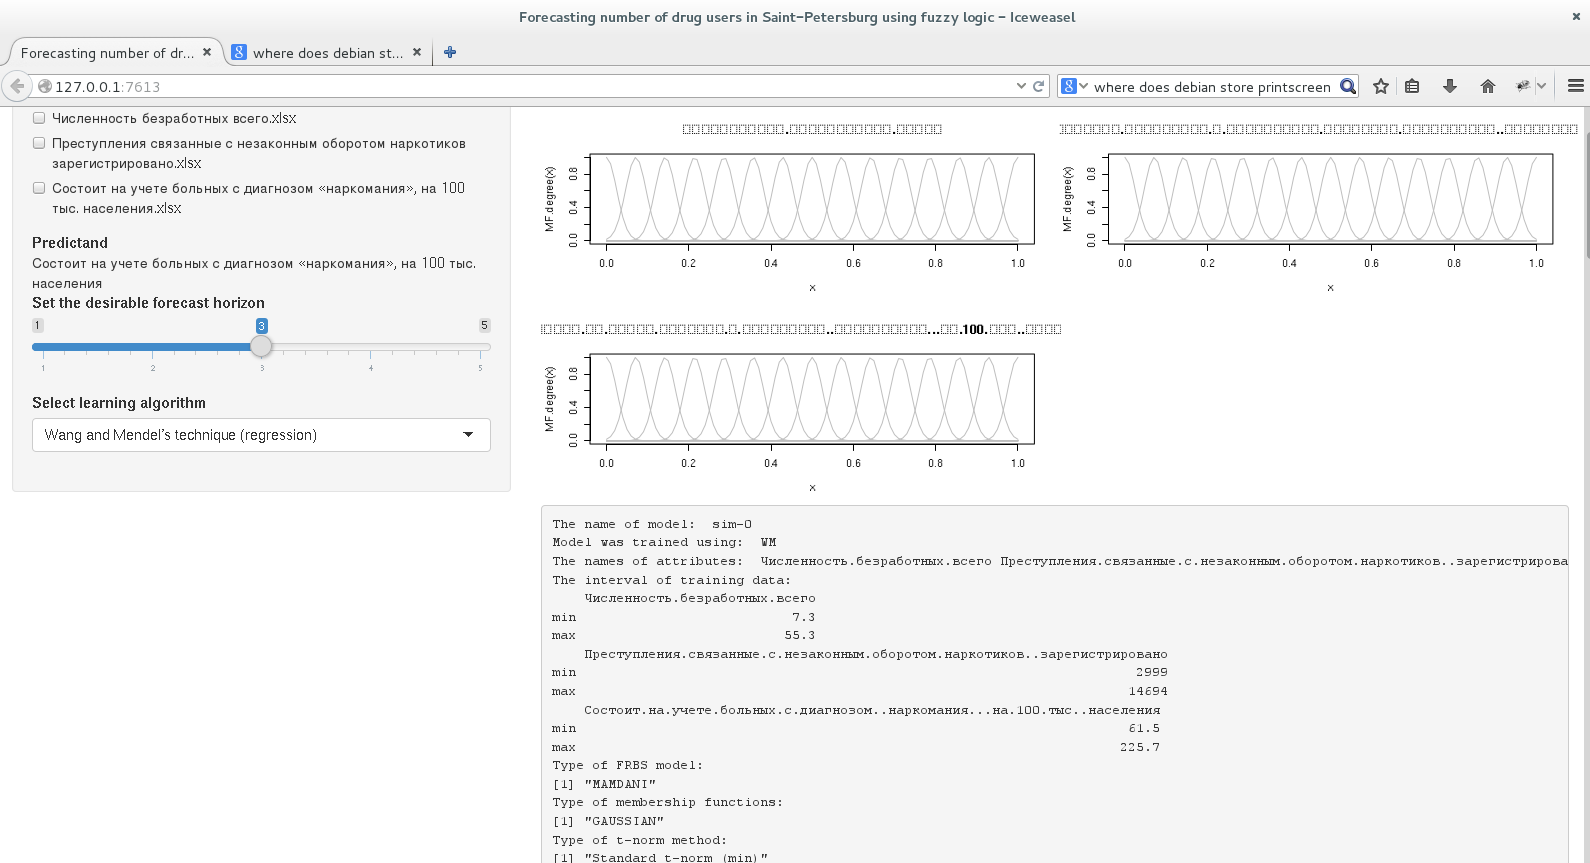
\includegraphics{images/screenshot3.png}
    \caption{Вкладка 3. Свойства нечеткой модели}		
    \label{figure:screenshot3}
\end{figure}

